%%=============================================================================
%% Methodologie
%%=============================================================================

\chapter{Methodologie}
\label{ch:methodologie}
\lstset{
    tabsize = 4, %% Sets tab space width.
    showstringspaces = false, %% Prevents space marking in strings, string is defined as the text that is generally printed directly to the console.
    numbers = left, %% Displays line numbers on the left.
    commentstyle = \color{green}, %% Sets comment color.
    keywordstyle = \color{blue}, %% Sets  keyword color.
    stringstyle = \color{red}, %% Sets  string color.
    rulecolor = \color{black}, %% Sets frame color to avoid being affected by text color.
    basicstyle = \small \ttfamily , %% Sets listing font and size.
    breaklines = true, %% Enables line breaking.
    numberstyle = \tiny,
}

%%\begin{lstlisting}[language = Java , frame = trBL , firstnumber = last , escapeinside={(*@}{@*)}]
%%public class Factorial
%%{
%%public static void main(String[] args)
%%{   final int NUM_FACTS = 100;
%%for(int i = 0; i < NUM_FACTS; i++)
%%System.out.println( i + "! is " + factorial(i));
%%}
%%
%%public static int factorial(int n)
%%{   int result = 1;
%%for(int i = 2; i <= n; i++) (*@\label{for}@*)
%%result *= i;
%%return result;
%%}
%%}
%%\end{lstlisting}


%% TODO: Hoe ben je te werk gegaan? Verdeel je onderzoek in grote fasen, en
%% licht in elke fase toe welke stappen je gevolgd hebt. Verantwoord waarom je
%% op deze manier te werk gegaan bent. Je moet kunnen aantonen dat je de best
%% mogelijke manier toegepast hebt om een antwoord te vinden op de
%% onderzoeksvraag.
\section{Opzet project}
Het opzetten van een omgeving is per technologie verschillend. Elk heeft zijn eigen manier om data te verzenden en te ontvangen. Hieronder wordt eerst eens per technologie de implementatie getoond hoe we het project opgezet hebben. Daarna wordt er uitgelegd hoe we gaan testen welke nu de beste zal zijn. De reden waarom we specifiek deze technologieën gekozen hebben om te vergelijken kan opnieuw gelezen worden in de Stand van Zaken en de Inleiding.  

Deze klasse (Data.class) hergebruiken we in elke technologie. Deze klasse is het type van het bericht dat we verzenden.
\begin{lstlisting}[language = Java , frame = trBL , firstnumber = last , escapeinside={(*@}{@*)}]
@Getter
@AllArgsConstructor
@NoArgsConstructor
@ToString
public class Data {
    private int id;
    private String name;
    private String description;
}
     \end{lstlisting}
\subsection{Kafka}
In figuur 3.1 ziet u welke configuratie de topic heeft. Er wordt gebruik gemaakt van zes partities en de data wordt vier weken bijgehouden indien de berichten niet onmiddellijk gelezen worden. Na deze vier weken wordt de data verwijderd.
\begin{figure}[h!]
    \centering
    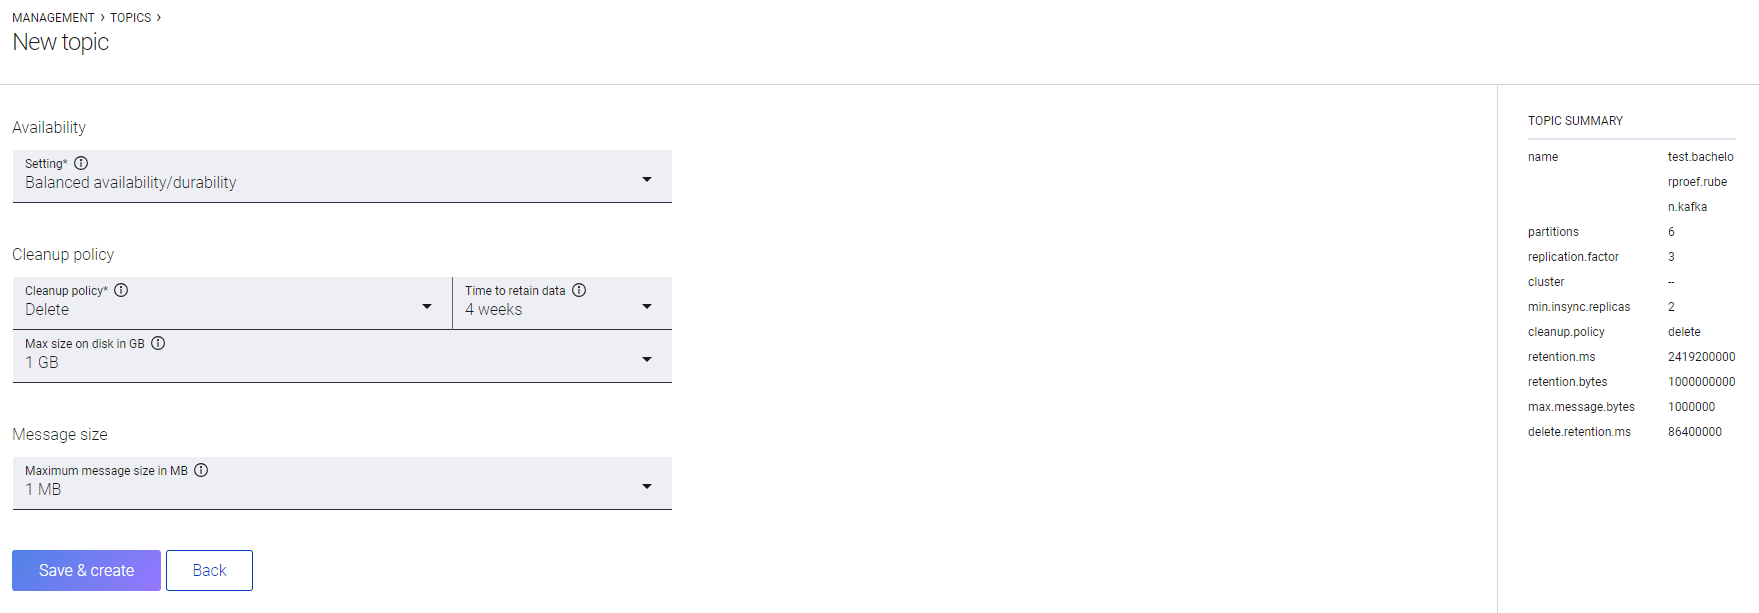
\includegraphics[width=140mm]{../kafkaConfig.png}
    \caption{Configuratie van de topic}
    
\end{figure}
\subsubsection{KafkaConfig}
Zo ziet de implementatie van de KafkaConfig.class eruit.
\begin{lstlisting}[language = Java , frame = trBL , firstnumber = last , escapeinside={(*@}{@*)}]
@Configuration
public class KafkaConfig {
    
    @Bean
    @Primary
    public KafkaProperties kafkaProperties(
    @Value("${kafka_key}") final String kafkaKey,
    @Value("${kafka_secret}") final String kafkaSecret
    
    ) {
        KafkaProperties kafkaProperties = new KafkaProperties();
       
        KafkaProperties.Producer producer = kafkaProperties.getProducer();
        
        producer.getProperties().put(ProducerConfig.KEY_SERIALIZER_CLASS_CONFIG, "org.apache.kafka.common.serialization.StringSerializer");
        producer.getProperties().put(ProducerConfig.VALUE_SERIALIZER_CLASS_CONFIG, "io.confluent.kafka.serializers.KafkaJsonSerializer");
        
        producer.getProperties().put(ProducerConfig.BOOTSTRAP_SERVERS_CONFIG, "pkc-412nj.europe-west1.gcp.confluent.cloud:9092");
        producer.getProperties().put(ProducerConfig.RETRIES_CONFIG, "2");
        producer.getProperties().put(ProducerConfig.ACKS_CONFIG, "all");
        producer.getProperties().put(ProducerConfig.RETRY_BACKOFF_MS_CONFIG, "1000");
        producer.getProperties().put(ProducerConfig.REQUEST_TIMEOUT_MS_CONFIG, "30000");
        producer.getProperties().put(ProducerConfig.LINGER_MS_CONFIG, "200");
        kafkaProperties.getProperties().put(SslConfigs.SSL_ENDPOINT_IDENTIFICATION_ALGORITHM_CONFIG, "https");
        kafkaProperties.getProperties().put(SaslConfigs.SASL_MECHANISM, "PLAIN");
        kafkaProperties.getProperties().put("request.timeout.ms", "20000");
        kafkaProperties.getProperties().put("retry.backoff.ms", "500");
        kafkaProperties.getProperties().put(SaslConfigs.SASL_JAAS_CONFIG, "org.apache.kafka.common.security.plain.PlainLoginModule required username=\""
        + kafkaKey + "\" password=\"" + kafkaSecret + "\";");
        kafkaProperties.getProperties().put("security.protocol", "SASL_SSL");
        
        
        
        return kafkaProperties;
    }
    \end{lstlisting}
    
    \subsubsection{KafkaPublisher}
    De KafkaPublisher.class is verantwoordelijk om de berichten te versturen naar de topic. De naam van de topic is meegegeven met het attribuut topicName. De kafkaTemplate wordt gebruikt om de berichten effectief mee te versturen. Het versturen zelf gebeurd wanneer de methode publish opgeroepen wordt. Deze methode maakt enkele berichten aan en verstuurd ze via de kafkaTemplate naar de topic die meegegeven is in het attribuut topicName.
        \begin{lstlisting}[language = Java , frame = trBL , firstnumber = last , escapeinside={(*@}{@*)}]
    @Component
    public class KafkaPublisher {
        
        private KafkaTemplate kafkaTemplate;
        private String topicName;
        
        public KafkaPublisher(KafkaTemplate kafkaTemplate,
        @Value("${kafka.topic.name}") String topicName) {
            this.kafkaTemplate = kafkaTemplate;
            this.topicName = topicName;
        }
        
        public void publish(List<Data> dataList) {
            for (Data data : dataList) {
                Message<Data> message = MessageBuilder.withPayload(data)
                .setHeader(KafkaHeaders.MESSAGE_KEY, String.valueOf(data.getId()))
                .setHeader(KafkaHeaders.TOPIC, topicName)
                .build();
                
                kafkaTemplate.send(message);
                System.out.println(message);
            }
        }
    }
     \end{lstlisting}
\subsection{RabbitMq}

\subsection{Google Pub/Sub}
\subsubsection{GooglePubSubConfig}
Zo ziet de GooglePubSubConfig.class eruit. Er worden twee kanalen aangemaakt van het type MessageChannel. Deze kanalen worden gebruikt om een bericht van een topic te lezen of verzenden.
        \begin{lstlisting}[language = Java , frame = trBL , firstnumber = last , escapeinside={(*@}{@*)}]
@Configuration
public class GooglePubSubConfig {
    @Bean("bachelorproef-channel-input")
    public MessageChannel createDeviceEventChannelInput() {
        return new DirectChannel();
    }
    
    @Bean("bachelorproef-channel-output")
    public MessageChannel createDeviceEventChannelOutput() {
        return new DirectChannel();
    }
    
    @Bean
    public PubSubInboundChannelAdapter createDeviceChannelAdapter(
    PubSubOperations pubSubTemplate,
    @Value("${pubsub.subscription}") String subsciptionName,
    @Qualifier("bachelorproef-channel-input") MessageChannel inputChannel,
    @Value("${pubsub.autostartup}") Boolean autoStart) {
        
        final PubSubInboundChannelAdapter adapter = new PubSubInboundChannelAdapter(pubSubTemplate, subsciptionName);
        adapter.setOutputChannel(inputChannel);
        adapter.setAckMode(AckMode.AUTO);
        adapter.setPayloadType(Event.class);
        adapter.setAutoStartup(autoStart);
        return adapter;
    }
    
    @Bean
    @ServiceActivator(inputChannel = "bachelorproef-channel-output")
    public MessageHandler messageSender(
    PubSubOperations pubsubTemplate,
    @Value("${pubsub.topic}") String topicName
    ) {
        return new PubSubMessageHandler(pubsubTemplate, topicName);
    }
    
    @Bean
    public JacksonPubSubMessageConverter createJacksonMessageConverter(final ObjectMapper objectMapper) {
        return new JacksonPubSubMessageConverter(objectMapper);
    }
    
}
     \end{lstlisting}
\subsubsection{GooglePubSubPublisher}
Deze klasse heeft maar één methode, namelijk publishData. Deze methode verstuurd het Data-object naar de topic via het kanaal \emph{bachelorproef-channel-output}. Er hoeft geen implementatie te zijn van deze methode, het spring-framework regelt al het andere werk in jouw plaats.
        \begin{lstlisting}[language = Java , frame = trBL , firstnumber = last , escapeinside={(*@}{@*)}]
@MessagingGateway(defaultRequestChannel = "bachelorproef-channel-output")
@Component
public interface GooglePubSubPublisher {
    void publishData(Data data);
    
}
     \end{lstlisting}
\section{Onderzoek}

